\chapter{Практичні результати}

У четвертому розділі представлено практичні результати
застосування алгоритму дифузії з сегментацією
та без із зазначенням вхідних даних.

\section{Практичні результати}

Вихідні зображення для побудови карти глибин
за допомогою описаних алгоритмів були взяті з набору стереопар,
зроблених в Мідлберійському коледжі в 2001~\cite{middlebury:ds:2001},
2003~\cite{middlebury:ds:2003}
та 2006~\cite{middlebury:ds:2006:1}~\cite{middlebury:ds:2006:2} роках.
На рисунку \ref{fig:stereopair:left} наведені ліві зображення зі стереопар,
для яких будувались карти глибин в даному розділі дисертації.
На рисунку \ref{fig:stereopair:right}
наведені праві зображення з тих же стереопар.

\begin{figure}[h]
\centering
    \begin{subfigure}[t]{0.32\textwidth}
        \centering
        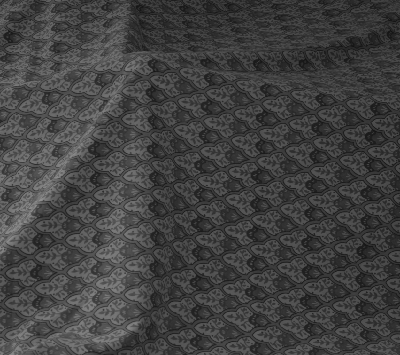
\includegraphics[width=\textwidth]{images/cloth_left}
        \caption{Тканина (Cloth1), $400 \times 355$ пікселів}
        \label{fig:cloth:left}
    \end{subfigure}
    \hfill
    \begin{subfigure}[t]{0.32\textwidth}
        \centering
        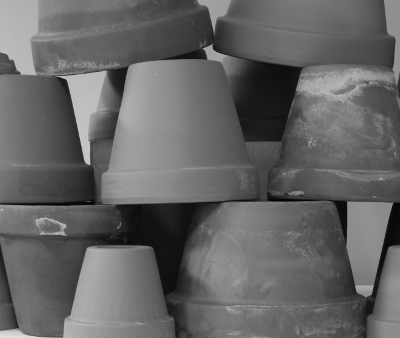
\includegraphics[width=\textwidth]{images/pots_left}
        \caption{Квіткові горщики (Flowerpots), $400 \times 338$ пікселів}
        \label{fig:flowerpots:left}
    \end{subfigure}
    \hfill
    \begin{subfigure}[t]{0.32\textwidth}
        \centering
        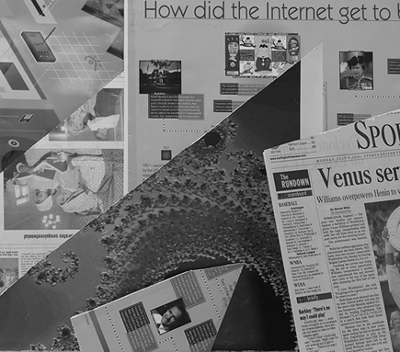
\includegraphics[width=\textwidth]{images/poster_left}
        \caption{Плакат (Poster), $400 \times 352$ пікселяв}
        \label{fig:poster:left}
    \end{subfigure}
    \caption{Ліві зображення стереопар}
    \label{fig:stereopair:left}
\end{figure}

\begin{figure}[h]
\centering
    \begin{subfigure}[t]{0.32\textwidth}
        \centering
        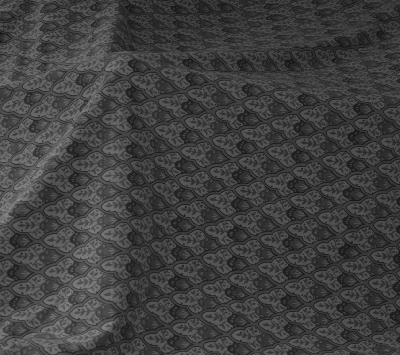
\includegraphics[width=\textwidth]{images/cloth_right}
        \caption{Тканина (Cloth1), $400 \times 355$ пікселів}
        \label{fig:cloth:right}
    \end{subfigure}
    \hfill
    \begin{subfigure}[t]{0.32\textwidth}
        \centering
        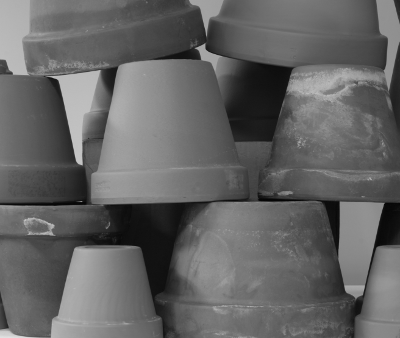
\includegraphics[width=\textwidth]{images/pots_right}
        \caption{Квіткові горщики (Flowerpots), $400 \times 338$ пікселів}
        \label{fig:flowerpots:right}
    \end{subfigure}
    \hfill
    \begin{subfigure}[t]{0.32\textwidth}
        \centering
        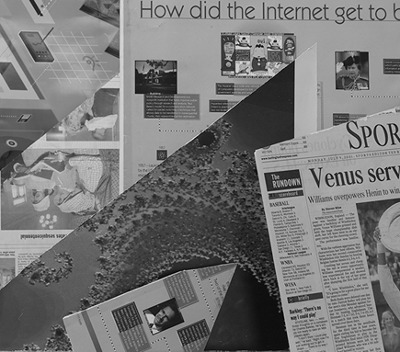
\includegraphics[width=\textwidth]{images/poster_right}
        \caption{Плакат (Poster), $400 \times 352$ пікселів}
        \label{fig:poster:right}
    \end{subfigure}
    \caption{Праві зображення стереопар}
    \label{fig:stereopair:right}
\end{figure}

На рисунку \ref{fig:result:pixel} зображені карти глибин,
отримані за допомогою алгоритму дифузії,
де кожній долі графу відповідає один піксель,
як описано в другому розділі дисертації.
Для кожного зображення вказано кількість ітерацій, зроблений алгоритмом дифузії,
час виконання всіх ітерацій, а також кількість міток $\left| D \right|$ в графі.

\begin{figure}[h]
\centering
    \begin{subfigure}[t]{0.32\textwidth}
        \centering
        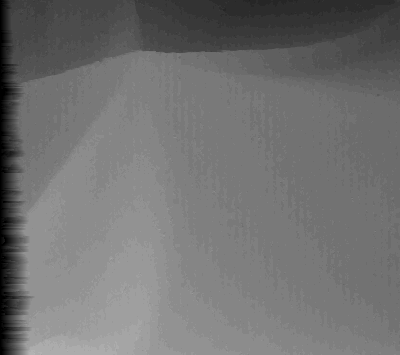
\includegraphics[width=\textwidth]{images/cloth_pixel_based_stereo}
        \caption{$2'400$ ітерацій, $5$ годин $40$ хвилин, $\left| D \right| = 40$}
        \label{fig:cloth:pixel}
    \end{subfigure}
    \hfill
    \begin{subfigure}[t]{0.32\textwidth}
        \centering
        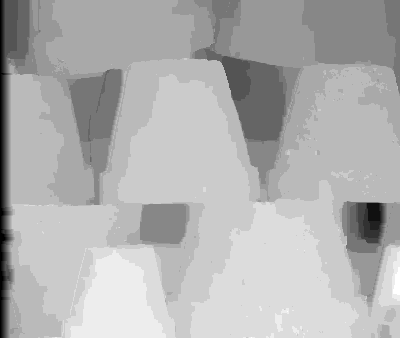
\includegraphics[width=\textwidth]{images/pots_pixel_based_stereo}
        \caption{$2'800$ ітерацій, $1$ година $20$ хвилин, $\left| D \right| = 16$}
        \label{fig:flowerpots:pixel}
    \end{subfigure}
    \hfill
    \begin{subfigure}[t]{0.32\textwidth}
        \centering
        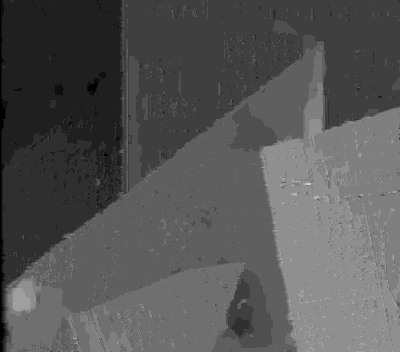
\includegraphics[width=\textwidth]{images/poster_pixel_based_stereo}
        \caption{$1'600$ ітерацій, $46$ хвилин, $\left| D \right| = 16$}
        \label{fig:poster:pixel}
    \end{subfigure}
    \caption{Карти глибин, отримані алгоритмом дифузії без сегментації зображення}
    \label{fig:result:pixel}
\end{figure}

На рисунку \ref{fig:result:superpixel} зображені карти глибин,
отримані за допомогою алгоритму дифузії з сегментацією зображення,
що описана в попередньому розділі дисертації,
з розміром комірок $5$ на $5$ пікселів.
Для кожного зображення вказано кількість ітерацій, зроблений алгоритмом дифузії,
час виконання всіх ітерацій, а також кількість міток $\left| D \right|$ в графі.
Отримані досить гладкі карти глибин,
однак видніються неточності на краях об'єктів.

\begin{figure}[h]
\centering
    \begin{subfigure}[t]{0.32\textwidth}
        \centering
        
\includegraphics[width=\textwidth]{images/cloth_superpixel_based_stereo}
        \caption{$100$ ітерацій, $19$ хвилин, $\left| D \right| = 40$}
        \label{fig:cloth:superpixel}
    \end{subfigure}
    \hfill
    \begin{subfigure}[t]{0.32\textwidth}
        \centering
        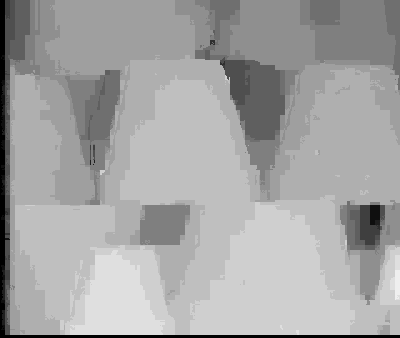
\includegraphics[width=\textwidth]{images/pots_superpixel_based_stereo}
        \caption{$450$ ітерацій, $15$ хвилин, $\; \left| D \right| = 16$}
        \label{fig:flowerpots:superpixel}
    \end{subfigure}
    \hfill
    \begin{subfigure}[t]{0.32\textwidth}
        \centering
        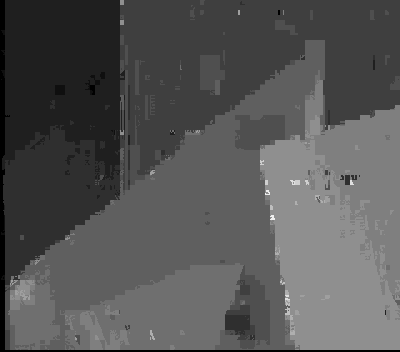
\includegraphics[width=\textwidth]{images/poster_superpixel_based_stereo}
        \caption{$400$ ітерацій, $14$ хвилин, $\; \left| D \right| = 16$}
        \label{fig:poster:superpixel}
    \end{subfigure}
    \caption{Карти глибин, отримані алгоритмом дифузії після сегментації зображення}
    \label{fig:result:superpixel}
\end{figure}

Для порівняння на рисунку \ref{fig:result:dynamic}
наведені карти глибин,
отримані з тими самими штрафними функціями
та значеннями параметрів за допомогою динамічного програмування,
де для кожного рядка зображення карта глибин шукається незалежно.
Хоча алгоритм і працює дуже швидко,
на отриманих картах глибин чітко видно горизонтальні лінії,
які є результатом того, що всі рядки зображення обробляються незалежно.
Таким чином, не алгоритм не враховує гладкість об'єктів.
Даний метод описано в першому розділі дисертації.

\begin{figure}[h]
\centering
    \begin{subfigure}[t]{0.32\textwidth}
        \centering
        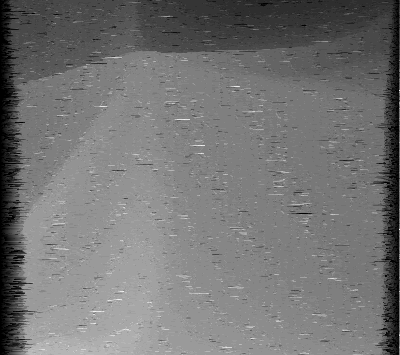
\includegraphics[width=\textwidth]{images/cloth_dynamic_result}
        \caption{$1.825$ секунди}
        \label{fig:cloth:result:dynamic}
    \end{subfigure}
    \hfill
    \begin{subfigure}[t]{0.32\textwidth}
        \centering
        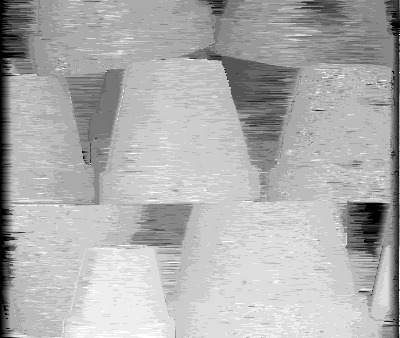
\includegraphics[width=\textwidth]{images/pots_dynamic_result}
        \caption{$0.792$ секунди}
        \label{fig:flowerpots:result:dynamic}
    \end{subfigure}
    \hfill
    \begin{subfigure}[t]{0.32\textwidth}
        \centering
        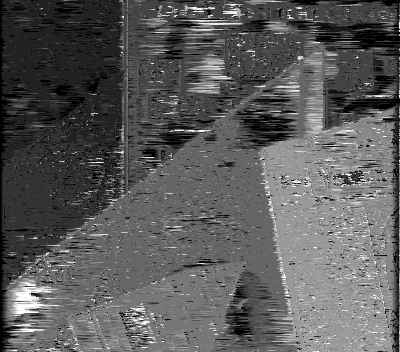
\includegraphics[width=\textwidth]{images/poster_dynamic_result}
        \caption{$0.83$ секунди}
        \label{fig:poster:result:dynamic}
    \end{subfigure}
    \caption{Карти глибин, отримані за допомогою динамічного програмування}
    \label{fig:result:dynamic}
\end{figure}

На рисунку \ref{fig:ground:truth}
наведені істинні синтезовані карти глибин,
надані разом за набором стереопар.
Карти глибин, отримані алгоритмом дифузії не є такими гладкими,
як ідеальні карти глибин.
Для підвищення гладкості карт глибин та позбавлення від артефактів
після застосування алгоритмів стереобачення
часто використовують згладжуючі фільтри та інші методи обробки карти глибин
\cite{refinement}.

% TODO: small overview of refinement method from paper as an example

% TODO: examples of refinement from paper

\begin{figure}[h]
\centering
    \begin{subfigure}[t]{0.32\textwidth}
        \centering
        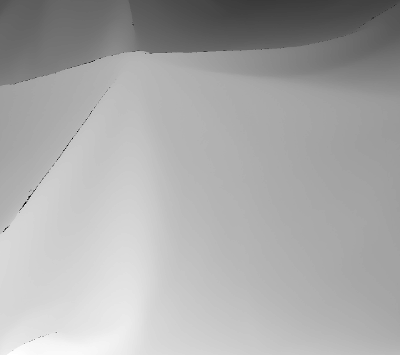
\includegraphics[width=\textwidth]{images/cloth_ground_truth}
        \caption{Тканина (Cloth1)}
        \label{fig:cloth:ground:truth}
    \end{subfigure}
    \hfill
    \begin{subfigure}[t]{0.32\textwidth}
        \centering
        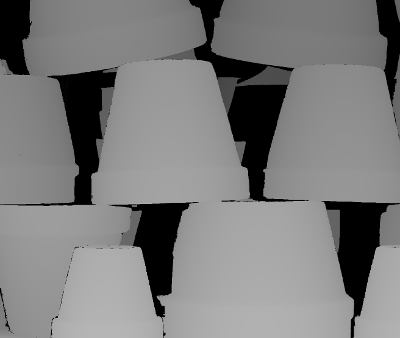
\includegraphics[width=\textwidth]{images/pots_ground_truth}
        \caption{Квіткові горщики (Flowerpots)}
        \label{fig:flowerpots:ground:truth}
    \end{subfigure}
    \hfill
    \begin{subfigure}[t]{0.32\textwidth}
        \centering
        
\includegraphics[width=\textwidth]{images/poster_ground_truth}
        \caption{Плакат (Poster)}
        \label{fig:poster:ground:truth}
    \end{subfigure}
    \caption{Істинні карти глибин}
    \label{fig:ground:truth}
\end{figure}

В якості штрафної функції для вершин $f$
в даній роботі використовувався модуль різниці
інтенсивностей відповідних пікселів на двох зображеннях
\begin{equation*}
    f_{\left(x, y \right)} \left( d \right) =
    \left| L \left(x, y \right) - R \left(x - d, y \right) \right|,
\end{equation*}
$\left(x, y \right) \in T$, $d \in D$,
а в якості штрафної функції для дужок $g$~---~модуль різниці вибраних зсувів
$d \in D$ та $d' \in D$ в сусідніх об'єктах графу
\begin{equation*}
    g_{\left(x, y \right), \left(x', y' \right)} \left(d, d' \right) =
    \alpha \cdot \left| d - d' \right|,
\end{equation*}
де $\left(\left(x, y \right), \left(x', y' \right) \right) \in \mathcal{N}$,
а $\alpha = 1.4$~---~коефіцієнт згладжування,
підібраний експериментальним шляхом.

% TODO: Prove that g is supermodular

Додатково були введені обмеження на можливі мітки в кожному об'єкті:
для об'єкта $\left( x, y \right) \in T$ з горизонтальною координатою $x$
не може бути обраний зсув $d \in D$, такий що $d > x$,
який би перевів горизонтальну координату пікселя у від'ємне число $x - d < 0$.
Дані обмеження були введені за допомогою штрафної функції $f$
\begin{equation*}
    f_{\left(x, y \right)} \left( d \right) =
    \begin{cases}
        \left| L \left(x, y \right) - R \left(x - d, y \right) \right|,
            & x \ge d, \\
        + \infty, & x < d.
    \end{cases}
\end{equation*}

% TODO: image for max possible disparity in image line

Також були накладені обмеження на зсуви в сусідніх об'єктах по горизонталі:
$d' \le d + 1$, де $d \in D$~---~мітка в об'єкті $\left(x, y \right) \in T$,
$d'$~---~мітка в об'єкті
$\left(x', y' \right) \in \mathcal{N} \left(x, y \right)$,
такому що $x' = x + 1$.

% TODO: add image

% Алгоритм был реализован на языке программиро-
% вания Rust. В ходе работы был использован компью-
% тер с процессором Intel(R) Core(TM) i5-7400 и ОЗУ
% DDR4 2133MHz.

\section*{Висновки до розділу 4}
\addcontentsline{toc}{section}{Висновки до розділу 4}

% TODO: Add conclusions
